\section*{Exercice 173 -- SLCI Calculs}
% CCS TSI 2015

\setcounter{exo}{0}


L'étude suivante consiste à obtenir un modèle simplifié de la boucle
d'asservissement de vitesse (figure suivante) au regard des réglages effectués
et de l'influence d'une perturbation de type échelon sur le dosseret. En
effet, vu la courte durée des sollicitations, la perturbation sur le
dosseret, dont l'origine peut être une action du spectateur sur ses
muscles cervicaux, peut être modélisée par un échelon.


\begin{center}
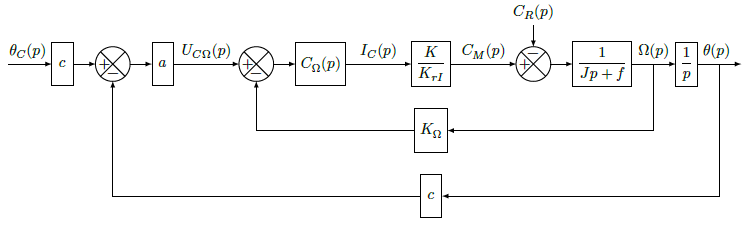
\includegraphics[width=1.0\linewidth]{044_01.png}
\textit{Modèle de la boucle d'asservissement de vitesse \label{fig13}}
\end{center}


 On a \(C_{\Omega}\left( p \right) = k_{1}\left( 1 + \dfrac{1}{T_{1}p} \right)\). De plus : 
$K = \SI{0,115}{N.m.A^{-1}}$;
$R = \SI{1}{\Omega}$;
$L = \SI{1,1}{mH}$;
$K_{rI}= \SI{0,5}{V. A^{-1}}$;
%	h = 6
$r = 1/50$;
$f = \SI{4.1e-4}{N.m.s.rad^{-1}}$;
$J=\SI{0,16e-3}{kg.m^{2}}$.

 
 



\subparagraph{}\textit{Exprimer la fonction de transfert de la boucle de vitesse
  \(H_{\Omega}\left( p \right) = \Omega(p)/U_{C\Omega}(p)\), lorsque
  \(C_{R}\left( p \right) = 0\). Le résultat sera mis sous une forme canonique.}

\ifprof
\begin{corrige}~\\

$H_{\Omega}(p)=\dfrac{k_{1}\left( 1 + \dfrac{1}{T_{1}p} \right)\dfrac{K}{K_{rI}}\dfrac{1}{Jp+f}}{1+ K_{\Omega}k_{1}\left( 1 +\dfrac{1}{T_{1}p} \right)\dfrac{K}{K_{rI}}\dfrac{1}{Jp+f}}$
$=\dfrac{k_{1}\left( 1 + T_{1}p \right)K}{T_{1}p K_{rI}\left(Jp+f\right) + K_{\Omega}k_{1}\left(1+ T_{1}p\right) K}$

~\\

$=\dfrac{\dfrac{Kk_{1}}{K_{\Omega}k_{1}K}\left( 1 + T_{1}p \right)}{\dfrac{T_{1} K_{rI}J}{K_{\Omega}k_{1}K}p^2+\left(\dfrac{fT_{1} K_{rI}}{K_{\Omega}k_{1}K}+\dfrac{K_{\Omega}k_{1}T_{1}K}{K_{\Omega}k_{1}K}\right)p + 1 }$
$H_{\Omega}(p)=\dfrac{\dfrac{1}{K_{\Omega}}\left( 1 + T_{1}p \right)}{\dfrac{T_{1} K_{rI}J}{K_{\Omega}k_{1}K}p^2+\left(\dfrac{f K_{rI}}{K_{\Omega}k_{1}K}+1\right)T_{1}p + 1 }$

\end{corrige}
\else
\fi

\subparagraph{}\textit{$T_1$ étant égal à $J/f$, montrer alors que
  la fonction de transfert en boucle fermée peut se mettre sous la forme
  \(\dfrac{b}{\tau p + 1}\). Calculer les valeurs numériques des termes
  \emph{b} et \emph{$\tau$}.}

\ifprof
\begin{corrige}~\\

\footnotesize

On a 
$H_{\Omega}(p)=\dfrac{\dfrac{1}{K_{\Omega}}\left( 1 + \dfrac{J}{f}p \right)}{\dfrac{\dfrac{J}{f} K_{rI}J}{K_{\Omega}k_{1}K}p^2+\left(\dfrac{f K_{rI}}{K_{\Omega}k_{1}K}+1\right)\dfrac{J}{f}p + 1 }$
$=\dfrac{\left( f + Jp \right)}{\dfrac{ K_{rI}J^2}{k_{1}K}p^2+\left(\dfrac{f K_{rI}}{k_{1}K}+K_{\Omega}\right)Jp + fK_{\Omega}}$

$=\dfrac{\left( f + Jp \right)k_{1}K}{ K_{rI}J^2p^2+\left(f K_{rI}+K_{\Omega}k_{1}K\right)Jp + fK_{\Omega}k_{1}K}$


On a :
$\Delta =\left(f K_{rI}+K_{\Omega}k_{1}K\right)^2J^2 -4 fK_{\Omega}k_{1}KK_{rI}J^2 $ 
$=\left(f^2 K_{rI}^2+K_{\Omega}^2k_{1}^2K^2+2f K_{rI}K_{\Omega}k_{1}K\right)J^2 -4 fK_{\Omega}k_{1}KK_{rI}J^2 $

$=\left(f^2 K_{rI}^2+K_{\Omega}^2k_{1}^2K^2-2f K_{rI}K_{\Omega}k_{1}K\right)J^2  $
$=\left(f K_{rI}-K_{\Omega}k_{1}K\right)^2J^2  $

On a donc 

$p_{12} = \dfrac{-\left(f K_{rI}+K_{\Omega}k_{1}K\right)J \pm \left(f K_{rI}-K_{\Omega}k_{1}K\right)J}{2 K_{rI}J^2}$, 

$p_{1} = \dfrac{-fJ K_{rI}-K_{\Omega}k_{1}KJ + fJ K_{rI}-K_{\Omega}k_{1}KJ}{2 K_{rI}J^2}$
$= -\dfrac{K_{\Omega}k_{1}K }{ K_{rI}J}$, 
$p_{2} = \dfrac{-fJ K_{rI}-K_{\Omega}k_{1}KJ -fJ K_{rI}+K_{\Omega}k_{1}KJ}{2 K_{rI}J^2}= -\dfrac{f }{J}$.

On a donc 

$H_{\Omega}(p)=\dfrac{J\left( \dfrac{f}{J} + p \right)k_{1}K}{\left(p+\dfrac{f }{J} \right)\left(p+\dfrac{K_{\Omega}k_{1}K }{ K_{rI}J} \right)}=\dfrac{Jk_{1}K}{p+\dfrac{K_{\Omega}k_{1}K }{ K_{rI}J} }$
$=\dfrac{\dfrac{ K_{rI}J^2}{K_{\Omega} } }{\dfrac{ K_{rI}J}{K_{\Omega}k_{1}K }p+1 }$

On a donc $b=\dfrac{ K_{rI}J^2}{K_{\Omega} }$ et $\tau =\dfrac{ K_{rI}J}{K_{\Omega}k_{1}K }$.

\normalsize
Autre solution : $b=\dfrac{1}{K_{\Omega}} = 20 \pi = \SI{62,8}{rad.s{-1}V^{-1}}$ et $\tau=\dfrac{K_{ri}J}{k_1KK_{\Omega}}=\SI{2,17e-3}{s}$.


\end{corrige}
\else
\fi

\subparagraph{}\textit{En déduire, à l'aide de la figure précédente, $\theta(p)/C_R(p)$
  lorsque $\theta_C(p)=0$. Calculer ensuite la valeur finale
  de $\theta(t)$ lorsque $c_R(t)$ est un échelon unitaire. %*******
  Conclure quant à l'action, en régime permanent, du correcteur
  proportionnel et intégral sur les effets d'une perturbation
  $c_R(t)$ de type échelon.}

\ifprof
\begin{corrige}~\\

\begin{center}
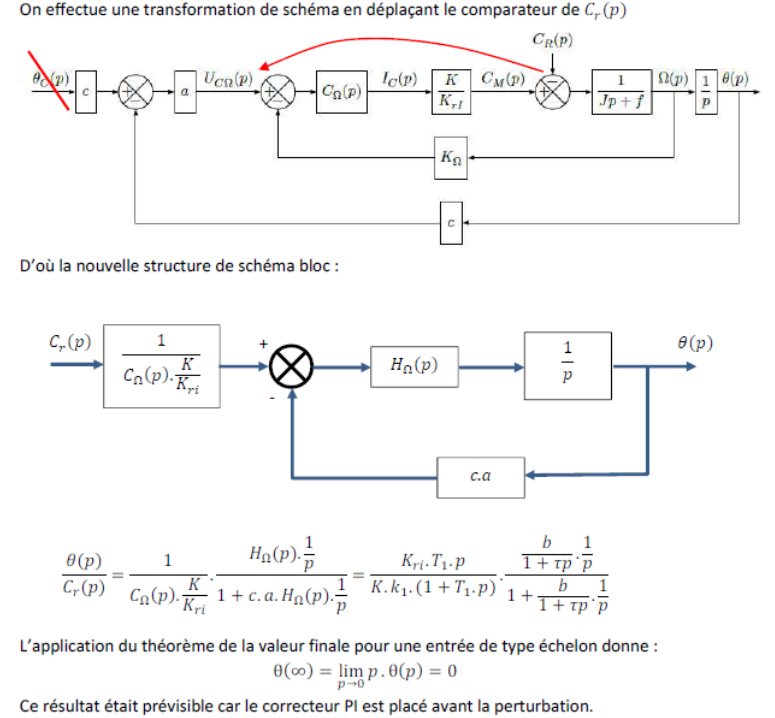
\includegraphics[width=\linewidth]{cor_01.png}
\end{center}

$\dfrac{\theta(p)}{C_r(p)}=\dfrac{1}{C_{\Omega}(p)\dfrac{K}{K_{ri}}}\dfrac{\dfrac{b}{1+\tau p}\dfrac{1}{p}}{1+\dfrac{abc}{1+\tau p}\dfrac{1}{p}}$ 
$=\dfrac{1}{ k_{1}\left( 1 + \dfrac{1}{T_{1}p} \right)\dfrac{K}{K_{ri}}}\dfrac{\dfrac{b}{1+\tau p}\dfrac{1}{p}}{1+\dfrac{abc}{1+\tau p}\dfrac{1}{p}}$

$=\dfrac{T_{1}K_{ri}p}{ k_{1}\left( T_{1}p + 1 \right)K}\cdot \dfrac{b}{p\left(1+\tau p \right)+abc}$

et $\lim\limits_{t\to\infty} \theta(t) = 1$.
\end{corrige}
\else
\fi